\documentclass[10pt,a4paper]{amsart}
\usepackage{amsmath,amssymb,amsthm,graphicx}
% Class-compatibility preamble for a reader excerpt of
%   Masuda-Thomas-Tonks-Vallette, "The diagonal of the associahedra", JEP 8 (2021), DOI 10.5802/jep.142.
%
% This file is the source directory's inherited layout adapter, unchanged except for one
% mechanical line: \smaller is declared with \providecommand instead of \newcommand because the
% wrapper class used for this excerpt (amsart) already defines \smaller as a font-size command.
% No mathematical macro, statement or proof step is added.
\usepackage{amsmath,amssymb,amsthm,xfrac,xspace,hyperref,graphicx,comment}
\excludecomment{DefTralics}

\providecommand{\bibliofont}{\small}
\newcommand{\ie}{i.e.,\xspace}
\newcommand{\eg}{e.g.,\xspace}
\newcommand{\etc}{etc.\xspace}
\newcommand{\cf}{cf.\xspace}
\newcommand{\resp}{resp.\xspace}
\providecommand{\smaller}{\small}
\newcommand{\Subsection}{\subsection}
\newcommand{\Subsubsection}{\subsubsection}
\newcommand{\skpt}{\smallskip}
\emergencystretch=3em
\numberwithin{equation}{section}\providecommand{\No}{}
\usepackage{mathrsfs}
\let\mathcal\mathscr
\usepackage{mathtools}
\newcommand{\Changel}{\mathcode`l="7160}
\newcommand{\Changelback}{\mathcode`l="716C}
\newcommand{\NoChangel}[1]{%
\expandafter\let\csname old\string#1\endcsname=#1
\let#1=\relax
\newcommand{#1}{\mathcode`l="716C\csname old\string#1\endcsname\mathcode`l="7160 }%
}
\def\mto{\mathchoice{\longmapsto}{\mapsto}{\mapsto}{\mapsto}}
\def\hto{\mathrel{\lhook\joinrel\to}}
\def\ltwoheadrightarrow{\longrightarrow\hspace*{-5mm}\longrightarrow}
\def\stwoheadrightarrow{\rightarrow\hspace*{-3mm}\rightarrow}
\def\twoheadrightarrow{\mathchoice{\ltwoheadrightarrow}{\stwoheadrightarrow}{\stwoheadrightarrow}{\stwoheadrightarrow}}
\def\To#1{\mathchoice{\xrightarrow{\textstyle\kern4pt#1\kern3pt}}{\stackrel{#1}{\longrightarrow}}{}{}}
\def\Hto#1{\mathrel{\lhook\joinrel\To{#1}}}
\newcommand{\sbullet}{{\scriptscriptstyle\bullet}}

\NoChangel{\log}
\NoChangel{\ln}
\NoChangel{\lim}
\NoChangel{\limsup}
\NoChangel{\liminf}
\NoChangel{\varlimsup}
\NoChangel{\varliminf}
\NoChangel{\varinjlim}
\NoChangel{\varprojlim}

\let\dpl\displaystyle
\let\ts\textstyle

\AtBeginDocument{%
\def\labelitemi{$\sbullet$}%
}

\usepackage{graphicx}
\usepackage{multirow}

\usepackage[noabbrev,capitalize]{cleveref}
\crefdefaultlabelformat{#2\textup{#1}#3}

\usepackage{tikz}
\usepackage{tikz-cd}
\tikzset{math3d/.style=
{x= {(-0.353cm,-0.353cm)}, z={(0cm,1cm)},y={(1cm,0cm)}}}
\tikzset{JLL3d/.style=
{x= {(0.4cm,-0.2cm)}, z={(0cm,1cm)},y={(-1cm,0cm)}}}

\theoremstyle{plain}
\newtheorem{proposition}{Proposition}
\newtheorem{theorem}{Theorem}
\newtheorem*{problem}{Problem}
\newtheorem{corollary}{Corollary}
\newtheorem{lemma}{Lemma}
\newtheorem{conjecture}{Conjecture}

\theoremstyle{definition}
\newtheorem{definition}{Definition}
\newtheorem{remark}{Remark}
\newtheorem{example}{Example}

\newcommand{\RR}{\mathbb{R}}
\newcommand{\ZZ}{\mathbb{Z}}
\newcommand{\ZP}{\mathbb{Z}_{>0}}
\newcommand{\K}{{K}}
\newcommand{\La}{\mathcal{L}}
\newcommand{\Tam}[1]{\mathrm{PBT}_{#1}}
\newcommand{\PT}[1]{\mathrm{PT}_{#1}}
\newcommand{\sC}{\mathcal{C}}
\newcommand{\PolySub}{\mathsf{Poly}}\NoChangel{\PolySub}
\newcommand{\Top}{\mathsf{Top}}
\newcommand{\CW}{\mathsf{CW}}
\newcommand{\sF}{\mathcal{F}}
\DeclareMathOperator{\tp}{top}
\DeclareMathOperator{\bm}{bot}
\DeclareMathOperator{\pr}{pr}
\DeclareMathOperator{\conv}{conv}
\DeclareMathOperator{\diam}{diam}
\newcommand{\ang}[1]{\langle #1\rangle}
\renewcommand{\No}{\mathcal{N}}
\newcommand{\Ve}{\mathcal{V}}
\newcommand{\Bool}[1]{\{0, 1\}^{#1}}
\newcommand{\sk}{\mathrm{sk}}
\DeclareMathOperator{\vol}{vol}\NoChangel{\vol}
\newcommand{\tr}{\mathrm{tr}}
\newcommand{\id}{\mathrm{id}}
\newcommand{\itd}[1]{\triangle^{(#1)}}
\DeclareMathOperator*{\colim}{\mathrm{colim}}
\DeclareMathOperator{\im}{\mathrm{Im}}
\newcommand{\abs}[1]{\lvert #1\rvert}
\DeclareMathOperator{\codim}{codim}

\newcommand{\TreeR}
{\vcenter{\hbox{
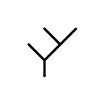
\begin{tikzpicture}[yscale=0.2,xscale=0.2]
\draw[thick] (0,-1)--(0,0) -- (2,2);
\draw[thick] (1,1)--(0,2) ;
\draw[thick] (0,0)--(-1,1) ;
\draw [fill] (0,-1) circle [radius=0.035];
\draw [fill] (2,2) circle [radius=0.035];
\draw [fill] (0,2) circle [radius=0.035];
\draw [fill] (-1,1) circle [radius=0.035];
\end{tikzpicture}}}}
\newcommand{\TreeL}
{\vcenter{\hbox{
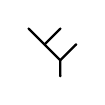
\begin{tikzpicture}[yscale=0.2,xscale=0.2]
\draw[thick] (0,-1)--(0,0) -- (-2,2);
\draw[thick] (-1,1)--(0,2) ;
\draw[thick] (0,0)--(1,1) ;
\draw [fill] (0,-1) circle [radius=0.035];
\draw [fill] (-2,2) circle [radius=0.035];
\draw [fill] (0,2) circle [radius=0.035];
\draw [fill] (1,1) circle [radius=0.035];
\end{tikzpicture}}}}
\newcommand{\TreeLL}
{\vcenter{\hbox{
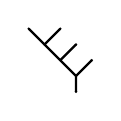
\begin{tikzpicture}[yscale=0.2,xscale=0.2]
\draw[thick] (0,-1)--(0,0) -- (-3,3);
\draw[thick] (-1,1)--(0,2) ;
\draw[thick] (-2,2)--(-1,3) ;
\draw[thick] (0,0)--(1,1) ;
\draw [fill] (0,-1) circle [radius=0.035];
\draw [fill] (-2,2) circle [radius=0.035];
\draw [fill] (0,2) circle [radius=0.035];
\draw [fill] (1,1) circle [radius=0.035];
\draw [fill] (-3,3) circle [radius=0.035];
\draw [fill] (-1,3) circle [radius=0.035];
\end{tikzpicture}}}}
\newcommand{\TreeLR}
{\vcenter{\hbox{
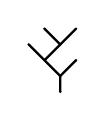
\begin{tikzpicture}[yscale=0.2,xscale=0.2]
\draw[thick] (0,-1)--(0,0) -- (-2,2);
\draw[thick] (-1,1)--(1,3) ;
\draw[thick] (0,0)--(1,1) ;
\draw[thick] (0,2)--(-1,3) ;
\draw [fill] (0,-1) circle [radius=0.035];
\draw [fill] (-2,2) circle [radius=0.035];
\draw [fill] (0,2) circle [radius=0.035];
\draw [fill] (1,1) circle [radius=0.035];
\draw [fill] (-1,3) circle [radius=0.035];
\draw [fill] (1,3) circle [radius=0.035];
\end{tikzpicture}}}}
\newcommand{\TreeRR}
{\vcenter{\hbox{
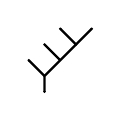
\begin{tikzpicture}[yscale=0.2,xscale=0.2]
\draw[thick] (0,-1)--(0,0) -- (3,3);
\draw[thick] (1,1)--(0,2) ;
\draw[thick] (2,2)--(1,3) ;
\draw[thick] (0,0)--(-1,1) ;
\draw [fill] (0,-1) circle [radius=0.035];
\draw [fill] (2,2) circle [radius=0.035];
\draw [fill] (0,2) circle [radius=0.035];
\draw [fill] (-1,1) circle [radius=0.035];
\draw [fill] (3,3) circle [radius=0.035];
\draw [fill] (1,3) circle [radius=0.035];
\end{tikzpicture}}}}
\newcommand{\TreeRL}
{\vcenter{\hbox{
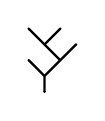
\begin{tikzpicture}[yscale=0.2,xscale=0.2]
\draw[thick] (0,-1)--(0,0) -- (2,2);
\draw[thick] (1,1)--(-1,3) ;
\draw[thick] (0,0)--(-1,1) ;
\draw[thick] (0,2)--(1,3) ;
\draw [fill] (0,-1) circle [radius=0.035];
\draw [fill] (2,2) circle [radius=0.035];
\draw [fill] (0,2) circle [radius=0.035];
\draw [fill] (-1,1) circle [radius=0.035];
\draw [fill] (1,3) circle [radius=0.035];
\draw [fill] (-1,3) circle [radius=0.035];
\end{tikzpicture}}}}
\newcommand{\TreeCC}
{\vcenter{\hbox{
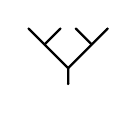
\begin{tikzpicture}[yscale=0.2,xscale=0.2]
\draw[thick] (0,-1)--(0,0) -- (-2.5,2.5);
\draw[thick] (-1.5,1.5)--(-0.5,2.5) ;
\draw[thick] (1.5,1.5)--(0.5,2.5) ;
\draw[thick] (0,0)--(2.5,2.5) ;
\draw [fill] (0,-1) circle [radius=0.035];
\draw [fill] (-2.5,2.5) circle [radius=0.035];
\draw [fill] (-0.5,2.5) circle [radius=0.035];
\draw [fill] (0.5,2.5) circle [radius=0.035];
\draw [fill] (2.5,2.5) circle [radius=0.035];
\end{tikzpicture}}}}
\newcommand{\TreeAL}
{\vcenter{\hbox{
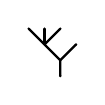
\begin{tikzpicture}[yscale=0.2,xscale=0.2]
\draw[thick] (0,-1)--(0,0) -- (-2,2);
\draw[thick] (-1,1)--(0,2) ;
\draw[thick] (0,0)--(1,1) ;
\draw[thick] (-1,1)--(-1,2) ;
\draw [fill] (0,-1) circle [radius=0.035];
\draw [fill] (-2,2) circle [radius=0.035];
\draw [fill] (0,2) circle [radius=0.035];
\draw [fill] (1,1) circle [radius=0.035];
\draw [fill] (-1,2) circle [radius=0.035];
\end{tikzpicture}}}}
\newcommand{\TreeRA}
{\vcenter{\hbox{
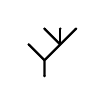
\begin{tikzpicture}[yscale=0.2,xscale=0.2]
\draw[thick] (0,-1)--(0,0) -- (2,2);
\draw[thick] (1,1)--(0,2) ;
\draw[thick] (0,0)--(-1,1) ;
\draw[thick] (1,1)--(1,2) ;
\draw [fill] (0,-1) circle [radius=0.035];
\draw [fill] (2,2) circle [radius=0.035];
\draw [fill] (0,2) circle [radius=0.035];
\draw [fill] (-1,1) circle [radius=0.035];
\draw [fill] (1,2) circle [radius=0.035];
\end{tikzpicture}}}}
\newcommand{\TreeAR}
{\vcenter{\hbox{
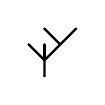
\begin{tikzpicture}[yscale=0.2,xscale=0.2]
\draw[thick] (0,-1)--(0,0) -- (2,2);
\draw[thick] (1,1)--(0,2) ;
\draw[thick] (0,0)--(-1,1) ;
\draw[thick] (0,0)--(0,1) ;
\draw [fill] (0,-1) circle [radius=0.035];
\draw [fill] (2,2) circle [radius=0.035];
\draw [fill] (0,2) circle [radius=0.035];
\draw [fill] (-1,1) circle [radius=0.035];
\draw [fill] (0,1) circle [radius=0.035];
\end{tikzpicture}}}}
\newcommand{\TreeLA}
{\vcenter{\hbox{
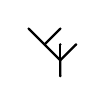
\begin{tikzpicture}[yscale=0.2,xscale=0.2]
\draw[thick] (0,-1)--(0,0) -- (-2,2);
\draw[thick] (-1,1)--(0,2) ;
\draw[thick] (0,0)--(1,1) ;
\draw[thick] (0,0)--(0,1) ;
\draw [fill] (0,-1) circle [radius=0.035];
\draw [fill] (-2,2) circle [radius=0.035];
\draw [fill] (0,2) circle [radius=0.035];
\draw [fill] (1,1) circle [radius=0.035];
\draw [fill] (0,1) circle [radius=0.035];
\end{tikzpicture}}}}
\newcommand{\TreeCA}
{\vcenter{\hbox{
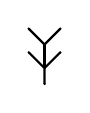
\begin{tikzpicture}[yscale=0.2,xscale=0.2]
\draw[thick] (0,-1)--(0,0) -- (-1,1);
\draw[thick] (0,1.5)--(1,2.5) ;
\draw[thick] (0,1.5)--(-1,2.5) ;
\draw[thick] (0,0)--(1,1) ;
\draw[thick] (0,0)--(0,1.5) ;
\draw [fill] (0,-1) circle [radius=0.035];
\draw [fill] (-1,1) circle [radius=0.035];
\draw [fill] (1,2.5) circle [radius=0.035];
\draw [fill] (-1,2.5) circle [radius=0.035];
\draw [fill] (1,1) circle [radius=0.035];
\draw [fill] (0,1) circle [radius=0.035];
\end{tikzpicture}}}}
\newcommand{\TreeC}
{\vcenter{\hbox{
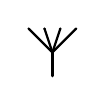
\begin{tikzpicture}[yscale=0.2,xscale=0.2]
\draw[thick] (0,-1.5)--(0,0);
\draw[thick] (0,0)--(1.5,1.5) ;
\draw[thick] (0,0)--(0.5,1.5) ;
\draw[thick] (0,0)--(-0.5,1.5) ;
\draw[thick] (0,0)--(-1.5,1.5) ;
\draw [fill] (0,-1.5) circle [radius=0.035];
\draw [fill] (1.5,1.5) circle [radius=0.035];
\draw [fill] (0.5,1.5) circle [radius=0.035];
\draw [fill] (-1.5,1.5) circle [radius=0.035];
\draw [fill] (-0.5,1.5) circle [radius=0.035];
\end{tikzpicture}}}}
\title{Canonical equivalence of the tight coherent diagonal subdivisions of normally equivalent positively oriented polytopes}
\author{Naruki Masuda, Hugh Thomas, Andy Tonks, Bruno Vallette}
\date{doi:10.5802/jep.142; CC BY 4.0}
\begin{document}
\maketitle
\setcounter{proposition}{5}
\noindent\textit{Editorial note.} All delivered mathematical text and both native TikZ figures are the authors' own, copied from the fixed publisher source; no statement, proof step or diagram was rewritten or removed.\par\medskip
\noindent\textit{Editorial note.} The publisher class cedram is replaced by a plain wrapper for this excerpt: the preamble is the source directory's existing class-compatibility adapter together with the authors' own macros, with the single mechanical change that the short macro smaller is declared with providecommand, since the wrapper class already defines it as a font-size command. No mathematical macro was introduced.\par\medskip
\noindent\textit{Editorial note.} The environment number printed here continues the authors' own per-type counter, so the statement appears as the sixth proposition of the article; its source label is Prop:NormalFan (source line 1121).\par\medskip
\noindent\textit{Editorial note.} Context blocks are the source definitions that the statement and its proof use: the well-oriented realization, the diagonal of a positively oriented polytope, the coherent-subdivision construction and coherent/tight subdivisions. They are marked as context and are not counted as this task's proof.\par\medskip
\noindent\textit{Allowed standard prerequisites (editorial).}\begin{itemize}
\item Standard convex polytope theory: faces, face lattices, normal cones and normal fans. Only the standard notion of normally equivalent polytopes (same normal fan) and elementary face/cone duality are assumed. The normal-cone characterisation of the diagonal image and the induced canonical equivalence of the two subdivisions remain the retained obligations.
\item Polar cones and the polar cone theorem for closed convex cones. The proof quotes the polar cone theorem to identify the polar of P-y with the normal cone of the face through y. That theorem is not re-proved; every step that involves the orientation vector, the diagonal map and the two subdivisions is the retained author argument.
\end{itemize}\medskip
\begin{definition}[Well-oriented realization of the associahedron]
A \emph{well-oriented reali\-zation of the associahedron} is a positively oriented polytope which realizes the associahedron and such that the orientation vector induces the Tamari lattice on the set of vertices.
\end{definition}

Before getting into specific argument on the associahedra, we construct a diagonal map $\triangle: P\to P\times P$ for any positively oriented polytope $(P, \vec v)$. Let $\tp_{\vec v} P$ (\resp $\bm_{\vec v} P$) denote the top (\resp bottom) vertex of $P$ with respect to the orientation vector $\vec v$.

\begin{definition}[Diagonal of a positively oriented polytope]\label{def:Diag}
The \emph{diagonal} of a positively oriented polytope $(P, \vec v)$ is defined by
\begin{align*}
\begin{array}{rlcl}
\triangle_{(P,\vec v)}\ : & P &\dpl\to &P\times P\\
&z & \dpl\mto&
\bigl(\bm_{\vec v}(P\cap \rho_z P),\, \tp_{\vec v}(P\cap \rho_z P)\bigr).
\end{array}
\end{align*}
\begin{figure}[htb]
\[
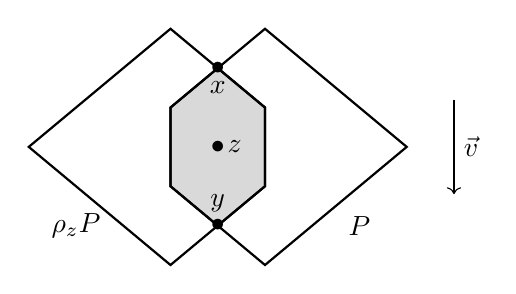
\begin{tikzpicture}[xscale=0.6, yscale=0.5]
\draw[thick] (1,3)--(-1,1)--(-1,-1)--(1,-3)--(4,0)--cycle;
\draw[thick] (-1,3)--(1,1)--(1,-1)--(-1,-3)--(-4,0)--cycle;

\draw[thick] (0,-2)--(-1,-1)--(-1, 1)--(0, 2)--(1, 1)--(1,-1)--cycle;
\draw[fill, opacity=0.15] (0,-2)--(-1,-1)--(-1, 1)--(0, 2)--(1, 1)--(1,-1)--cycle;

\draw[->] (5,1.2)--(5,-1.2);
\draw (5,0) node[right] {$\vec v$};
\draw (0,0) node {$\bullet$};
\draw (0,2) node {$\bullet$};
\draw (0,-2) node {$\bullet$};

\draw (0,0) node[right] {$z$};
\draw (0,1.9) node[below] {$x$};
\draw (0,-1.9) node[above] {$y$};

\draw (3,-2) node {$P$};
\draw (-3,-2) node {$\rho_z P$};
\end{tikzpicture}
\]
\caption{The diagonal map
$$\hspace*{-3cm}\triangle_{(P,\vec v)}(z)=\bigl(\bm_{\vec v}(P\cap \rho_z P),\, \tp_{\vec v}(P\cap \rho_z P)\bigr)=(x,y).$$}\label{Fig:Diag}
\end{figure}
\vspace*{-\baselineskip}
\end{definition}

Let $\beta$ be the middle-point map $P\times P\to P; (x,y)\mto \frac{x+y}{2}$.
With the notation $\pr_i$ for the projection to the $i$-th coordinate, we have $\pr_1\beta^{-1}(z)=\pr_2\beta^{-1}(z) = P\cap \rho_z P$.
The diagonal $\triangle_{(P,\vec v)}$ is a section of $\beta$ since $P\cap \rho_z P$ is symmetric with respect to the point $z$.

Let $\pi: Q\twoheadrightarrow P$ be an affine projection of polytopes with
$P\subset \RR^p$ and $Q\subset \RR^q$.
We~denote by $Q_z\coloneqq Q\cap \pi^{-1}(z)$ the fiber above $z\in P$.
To any linear form $\psi\in (\RR^q)^{\ast}$, we~associate a
collection
$\sF^\psi\subset \La(Q)$ as follows.
We first factor the affine projection~as\vspace*{-3pt}
\begin{align*}
\pi&=\mathrm{pr}\circ \tilde{\pi},& \text{where} \quad
\tilde{\pi}&\coloneqq (\pi, \psi): Q\twoheadrightarrow \tilde{P}\\
\tag*{and}
\mathrm{pr}&: \tilde{P}\twoheadrightarrow P;\, (z, t)\mto z,&
\text{where}\quad \tilde{P}&\coloneqq \big\{(\pi(x), \psi(x))\mid x\in Q\big\}\subset \RR^{p+1}.
\end{align*}
Next let $\La^{\downarrow}(\tilde P) \subset \La\big(\tilde{P}\big)$ be the subcomplex of lower faces, \ie $F\in \La^{\downarrow}(\tilde P)$ if and only if any $(z, t)\in F$ satisfies the equation
$t = \min \psi(Q_z)$. Since the preimage of any face by a projection of polytopes is again a face, this defines a collection\vspace*{-3pt}\enlargethispage{.5\baselineskip}%
\[\sF^\psi \coloneqq
\big\{Q\cap \tilde{\pi}^{-1}(F) \mid F\in \La^{\downarrow}(\tilde P)
\big\}
\subset \La(Q).\]
(This is in general not a polytopal complex since it is not stable under faces.)
In the case of the point $P=\{\ast\}$, the unique face contained in $\sF^\psi$ is by definition\vspace*{-3pt}
\[Q^\psi\coloneqq\{x\in Q \mid \psi (x) = \min \psi(Q)\}.\]

\begin{definition}[Coherent and tight subdivisions]\label{def:Coherent}
\begin{enumerate}
\item A subcollection $\sF\subset\La(Q)$ is called a \emph{coherent subdivision of $P$} when it is of the form $\sF^\psi$ for some $\psi\in (\RR^q)^{\ast}$.
\item A coherent subdivision $\sF$ is called \emph{tight} when, the faces $F$ and $\pi(F)$ have the same dimension, for every $F\in \sF$.
\end{enumerate}
\end{definition}

\begin{proposition}\label{Prop:NormalFan}
Suppose $P$ and $Q$ are normally equivalent polytopes,
\ie with same normal fans $\No_P=\No_Q$.
If $P$ and $Q$ are well-oriented by the same orientation vector $\vec v$,
then the tight coherent subdivisions
$\sF_{(P, \vec v)}$ and $\sF_{(Q, \vec v)}$ are combinatorially equivalent in a canonical way.
\end{proposition}

\begin{proof}
Normal equivalence of polytopes induces combinatorial equivalence
\[
\Phi: \La(P)\cong\La(Q).
\]
By the definition of the diagonal map, a pair of points $(x, y)\in P\times P$ is contained in the image $\im \triangle_P$ if and only if it satisfies the following condition:
there exists no vector $\vec w$ and positive number $\varepsilon >0$ with $\ang{\vec v, \vec w}>0$ and $x-\varepsilon \vec w, y+\varepsilon\vec w\in P$.
The latter conditions can be restated in terms of normal cones as follows. Recall that,
for any subset $C \subset \RR^n$, the polar cone $C^\star$ of $C$ is defined by
\[
C^\star \coloneqq\{ x\in \RR^n\mid \forall x\in C, \ \ang{x, y} \leq 0\}.
\]
The polar cone theorem asserts that $C^{\star \star}$ is the smallest closed convex cone which contains $C$.
By definition, $(P-y)^\star$ is the normal cone $\No_P(G)$ corresponding to the face which satisfies $y\in \mathring G$.
Applying the polar cone theorem to $C= P-y$, we obtain that $(P-y)^{\star\star} = \No_P(G)^\star$ is the set of vectors $\vec w$ such that $y+\varepsilon\vec w \in P$ for some $\varepsilon >0$.
Therefore if $x\in \mathring F$ and $y\in \mathring G$, the condition for $(x, y)\in \im \triangle_P$ is that
there exists no vector $\vec w$ such that
$\ang{\vec v, \vec w}>0$ and $\vec w\in -\No_P(F)^\star\cap \No_P(G)^\star$.
Since this condition depends only on the normal fan,
the map $\Phi\times \Phi: \La(P\times P)\to \La(Q\times Q)$ induces the canonical combinatorial equivalence $\sF_{(P, \vec v)}\cong \sF_{(Q, \vec v)}$.
\end{proof}

\end{document}
